\documentclass[12pt,a4paper]{article}
\usepackage[left=0.5cm, right=0.5cm, top=0.5cm, bottom=0.5cm]{geometry}
\usepackage{pgfpages}
\usepackage{pdfpages}
\usepackage{amsmath, amssymb, esint}
\usepackage{booktabs} % For tables
\usepackage{graphicx} % For images
\usepackage{tikz}
\usetikzlibrary{shapes, calc}
\usepackage{pdflscape}

\pgfpagesuselayout{4 on 1}[a4paper,border shrink=5mm]

\title{Physics Formula Sheet}
\author{402-0023-01L  Physics}
\date{2023/ 2024}

\begin{document}
	\maketitle
	
	\section*{Constants}
	\begin{tabular}{lll}
		\toprule
		Constant & Symbol & Value \\
		\midrule
		Speed of light & \( c \) & \( 3.00 \times 10^8 \) m/s \\
		Gravitational constant & \( G \) & \( 6.674 \times 10^{-11} \) N(m/kg)\(^2\) \\
		Planck's constant & \( h \) & \( 6.626 \times 10^{-34} \) J.s \\
		Mass of the electron & \( m_e \) & \( 9.10939 \times 10^{-31} \) kg \\
		Mass of the proton & \( m_p \) & \( 1.67262 \times 10^{-27} \) kg \\
		Charge of the electron & \(-e\) & \(-1.60218 \times 10^{-19} \) C \\
		Permittivity of free space & \(\epsilon_0\) & \( 8.85419 \times 10^{-12} \) C\(^2\)/J m \\
		Permeability of free space & \(\mu_0\) & \( 4 \pi \times 10^{-7} \) T m / A \\
		Boltzmann constant & \( k_B \) & \( 1.38066 \times 10^{-23} \) J/ K \\
		Avogadro's constant & \( N_A \) & \( 6.022 \times 10^{23} \) 1/mol \\
		\bottomrule
	\end{tabular}
	
	\section*{Oscillations}
	\begin{itemize}
		\item \textbf{Natural Frequency}: \( \sqrt{\frac{k}{m}}\)
		\item \textbf{Damping Ratio (\( \zeta \))}:
		\[
		\zeta = \frac{b}{b_c}
		\]
		where \( b_c = 2\sqrt{mk} \)
	\end{itemize}
	
	\subsection*{Quality Factor (Q factor)}
	
	The Q factor is a dimensionless parameter that describes the damping of an oscillator. It represents the energy stored to energy dissipated ratio. 
	\[
	Q = \frac{1}{2\zeta} = \frac{\omega_0}{\Delta \omega} = 2 \pi f \times \frac{\text{energy stored}}{\text{power loss}}
	\]
	where \( \Delta \omega \) is the bandwidth over which the energy is stored.
	
	\subsection*{Types of Oscillations}
	
	\begin{itemize}
		\item \textbf{Critically Damped (\( \zeta = 1 \))}: The system returns to equilibrium as quickly as possible without oscillating.
		\item \textbf{Overdamped (\( \zeta > 1 \))}: The system returns to equilibrium without oscillating but slower than the critically damped case.
		\item \textbf{Underdamped (\( \zeta < 1 \))}: The system oscillates about the equilibrium position with a frequency \( \omega_d \) given by:
		\[
		\omega_d = \omega_0 \sqrt{1 - \zeta^2}
		\]
	\end{itemize}
	
	\subsection*{General Solution}
	
	For a driven damped harmonic oscillator, the general solution can be expressed as:
	\[
	x(t) = e^{-\zeta \omega_0 t} \left( A \cos(\omega_d t) + B \sin(\omega_d t) \right)
	\]
	where \( A \) and \( B \) are constants determined by initial conditions.
	
\section*{Thermodynamics}

\begin{quote}
\textbf{0th law:} 
If two objects are in thermal equilibrium with a third object, then all three objects are in thermal equilibrium with each other.
\end{quote}
\begin{quote}
\textbf{1st law:} 
For any process concerning a given system, the change in internal energy \(\Delta U\) of that system is equal to the sum of the heat \( Q \) transferred to that system and the work \( W \) performed on that system.
\end{quote}

\begin{quote}
\textbf{2nd law:} 
\begin{itemize}
	\item \textbf{Carnot:} Wherever there exists a difference in temperature, motive power can be produced.
	\item \textbf{Kelvin:} It is impossible for a self-acting machine to convey heat from a colder body to a hotter one.
	\item \textbf{Clausius:} Heat cannot flow from a colder to a hotter body without another process occurring, connected therewith, simultaneously.
\end{itemize}
\end{quote}
\[
T = \left( \frac{\partial U}{\partial S} \right)_{V, N}
\]

Energy per mode: \( \langle E_\text{mode} \rangle = \frac{3}{2} k_B T \)

\[
Q = C \Delta T, \quad Q = \int_{T_1}^{T_2} C(T) \, dT
\]

\[
L = \frac{Q_\text{latent}}{m}, \quad \gamma = \frac{C_P}{C_V}, \quad dS = \frac{\delta Q_\text{rev}}{T}
\]

	\subsection*{Electrostatics and dynamics}
	\setlength{\parskip}{.8em} % Adjusts the spacing between lines
	
	\[
	\mathbf{F} = \sum_{i=1}^{N} \frac{q_0 q_i (\mathbf{r}-\mathbf{r_i})}{4\pi \epsilon_0 |\mathbf{r}-\mathbf{r_i}|^3}
	\]
	
	Torque: \( \mathbf{\tau} = \mathbf{p} \times \mathbf{E} \)
	
	Energy of a dipole: \( U(\theta) = -\mathbf{p} \cdot \mathbf{E} \)
	
	Gauss' law: \( \phi = \oiint_{S} \mathbf{E} \cdot d\mathbf{A} \)
	
	Potential: \( \Delta V \equiv \frac{\Delta U}{q} = - \int_{C} \mathbf{E} \cdot d\mathbf{l} \)
	
	Energy of a capacitor: \( U = \frac{Q^2}{2C} \)
	
	Current: \( I = \dot{Q} \)
	
	Potential: \( V_b - V_a = -\int_{a}^{b} \mathbf{E} \cdot d\mathbf{l} \)
	
	Kirchhoff's rules:
	1. \( \sum_{j, \text{loop}} \Delta V_j = 0 \)
	2. \( \sum_{j} I_{j, \text{into node}} = 0 \)
	
	Magnetic force: \( \mathbf{F} = q\mathbf{v} \times \mathbf{B} \)
	
	Cyclotron radius: \( r = \frac{mv}{qB} \)
	
	Biot-Savart: \( \mathbf{B} = \frac{\mu_0}{4 \pi} \cdot \frac{q \mathbf{v} \times \hat{r}}{r^2} \)
	
	Faraday's Law: \( \mathcal{E} = -\frac{d \phi_m}{dt} \)
	
	Self-inductance of a solenoid: \( L = \mu_0 n^2 A l \)
	
	Mutual inductance: \( \frac{\phi_{m1}}{N_1} = \frac{\phi_{m2}}{N_2} \)
	
	Impedance: \( Z_R = R, \, Z_C = \frac{1}{i \omega C}, \, Z_L = i \omega L \)
	
	\subsection*{Waves}
	\begin{align}
		\oint_{S} \mathbf{E} \cdot d\mathbf{A} &= \frac{Q_{\text{enc}}}{\epsilon_0} &\text{(Gauss's Law for Electricity)} \\
		\oint_{S} \mathbf{B} \cdot d\mathbf{A} &= 0 &\text{(Gauss's Law for Magnetism)} \\
		\oint_{C} \mathbf{E} \cdot d\mathbf{l} &= -\frac{d\Phi_{B}}{dt} &\text{(Faraday's Law)} \\
		\oint_{C} \mathbf{B} \cdot d\mathbf{l} &= \mu_0 I_{\text{enc}} + \mu_0 \epsilon_0 \frac{d\Phi_{E}}{dt} &\text{(Ampère's Law with Maxwell's addition)}
	\end{align}
	
	In electromagnetic waves, the ratio \( B_0 = \frac{E_0}{c} \) holds.
	
	Wavenumber: \( \omega = vk \)
	
	Compton wavelength: \( \lambda_c = \frac{h}{m_e c} \)
	
	De Broglie wavelength: \( \lambda_{\text{dB}} = \frac{h}{p} \)
	
	Heisenberg uncertainty relation: \( \Delta x \Delta p \geq \frac{h}{4\pi} \)
	
	Energy of a particle in a 1D box: \( E_n = \frac{h^2 n^2}{8L^2m} \)

	
	\section*{Quantum Mechanics}
	\begin{align*}
		\text{Time-dependent Schrodinger's Equation} & : i\hbar \frac{\partial}{\partial t} \Psi (\vec{x}, t) = [-\frac{\hbar^2}{2m}(\frac{\partial ^2}{\partial x^2} + \frac{\partial ^2}{\partial y ^2} + \frac{\partial^2}{\partial z^2}) + V(x)] \\
	\end{align*}
	
	\section*{Special relativity}
	Postulates of relativity and inertial reference frames:\\
	1: Absolute uniform motion cannot be detected.\\
	2: The speed of light in a vacuum is independent of the motion of the source.\\
	
	\subsection*{Doppler Shift}
	
	\textbf{Non-relativistic Doppler Shift:}
	\begin{align}
		f' &= f \left( \frac{c \pm v_{\text{observer}}}{c \pm v_{\text{source}}} \right) \quad \text{(for sound or slow-moving sources)}
	\end{align}
	
	\textbf{Relativistic Doppler Shift:}
	\begin{align}
		f' &= f \sqrt{\frac{1 + \beta}{1 - \beta}} \quad \text{(for motion towards the observer)} \\
		f' &= f \sqrt{\frac{1 - \beta}{1 + \beta}} \quad \text{(for motion away from the observer)}
	\end{align}
	where \( \beta = \frac{v_{\text{source}}}{c} \).
	
	\subsection*{Velocity Transformations in Special Relativity}
	
	For two observers in relative motion with velocity \( v \) along the x-axis:
	
	\begin{align}
		u'_{x} &= \frac{u_{x} + v}{1 + \frac{vu_{x}}{c^2}} \\
		u'_{y} &= \frac{u_{y}}{\gamma(1 + \frac{vu_{x}}{c^2})} \\
		u'_{z} &= \frac{u_{z}}{\gamma(1 + \frac{vu_{x}}{c^2})}
	\end{align}
	
	where \( \gamma = \frac{1}{\sqrt{1 - \frac{v^2}{c^2}}} \) is the Lorentz factor.
	
	\subsection*{Energy}
	$\text{E}_\text{total} = \gamma mc^2 = \sqrt{p^2c^2 + m^2c^4}, \text{E}_\text{rest} = mc^2$
	
	
	\section*{Mathematical equations}
	\subsection*{Trigonometric functions:}
	\begin{equation}
		\int \sin^n ax dx =
		\nonumber \\ 
		-\frac{1}{a}{\cos ax} \hspace{2mm}{_2F_1}\left[
		\frac{1}{2}, \frac{1-n}{2}, \frac{3}{2}, \cos^2 ax
		\right]
	\end{equation}
	\begin{equation}
		\int \sin ^2 ax dx = \frac{x}{2} - \frac{1}{4a} \sin 2ax + C
	\end{equation}
	\begin{equation}
		\int x \sin ^2 ax dx = \frac{x^2}{4} - \frac{x}{4a} \sin 2ax - \frac{1}{8a^2} \cos 2ax + C
	\end{equation}
	\begin{equation}
		\int x^2 \sin^2 x ax dx = \frac{x^3}{6} - (\frac{x^2}{4a} - \frac{1}{8a^3})\sin 2ax - \frac{x}{4a^2} \cos 2ax +C
	\end{equation}
	\begin{equation}
		\int \tan ax dx = - \frac{1}{a} \ln |\cos ax| + C = \frac{1}{a} \ln |\sec ax | +C
	\end{equation}
	\begin{equation}
		\int \frac{\cos ax}{x} dx = \ln |ax| + \sum_{1}^{\infty} (-)^k \frac{(ax)^{2k}}{2k (2k)!} +C
	\end{equation}
	\begin{equation}
		\int \cos ^2 ax dx = \frac{x}{2} + \frac{1}{4a} \sin 2ax + C
	\end{equation}
	\begin{equation}
		\int \sin^3 ax dx = \frac{\cos 3ax}{12a} - \frac{3 \cos ax}{4a} + C
	\end{equation}
	\begin{equation}
		\int \tan^2 x dx = \tan x -x +C
	\end{equation}
	\begin{equation}
		\int \sin ax \cos ax dx = - \frac{\cos^2 ax}{2a} + C
	\end{equation}
	\begin{equation}
		\int x \cos ax dx = \frac{\cos ax}{a^2} + \frac{x \sin ax}{a} + C
	\end{equation}
	\begin{equation}
		\int \cos ax dx = \frac{1}{a} \sin ax + C
	\end{equation}
	\begin{equation}
		\int x \sin ax dx = \frac{\sin ax }{a^2} -\frac{x \cos ax }{a} + C
	\end{equation}
	\begin{equation}
		\int (\sin ax) (\cos^n ax) dx = - \frac{1}{a ( n + 1)} \cos ^{n+1} ax + C
	\end{equation}
	
	
	\subsection*{Exponential functions:}
	
	
	
	
	
	\begin{equation}
		\int_{-\infty}^\infty e^{-ax^2}\hspace{1pt}\text{d}x = \frac{\sqrt{\pi}}{\sqrt{a}} \hspace*{3pt}(a > 0)
	\end{equation}
	\begin{equation}
		\int_{-\infty}^\infty x e^{-ax^2 + bx}\hspace{1pt}\text{d}x = \frac{\sqrt{\pi} b}{2a^{3/2}} e^{\frac{b^2}{4a}} \hspace{3pt}(\Re(a) > 0)
	\end{equation}
	\begin{equation}
		\int_{-\infty}^\infty x^n e^{-ax} \hspace{1pt} \text{d}x = \begin{cases}
			\dfrac{\Gamma (n+1)}{a^{n+1}} \hspace*{3pt} (n>-1, a>0)\\[.15in]
			\dfrac{n!}{a^{n+1}} \hspace*{3pt} (n=0,1,2,..., a>0)
		\end{cases}
	\end{equation}
	
	\begin{equation}
		\int_{-\infty}^\infty x^2 e^{-ax^2}\ {dx} = \frac{1}{2} \sqrt{\frac{\pi}{a^3}} \hspace*{3pt} (a > 0)
	\end{equation}
	\begin{equation}
		\int x e^{cx} dx = \left(\frac{x}{c}-\frac{1}{c^2}\right) e^{cx}
	\end{equation}
	\begin{equation}
		\int x^2 e^{cx} dx = \left(\frac{x^2}{c} - \frac{2x}{c^2} + \frac{2}{c^3}\right) e^{cx}
	\end{equation}
	\begin{equation}
		\int x^4 e^{-ax^2}\hspace{1pt} dx = \sqrt{\dfrac{\pi }{a}} \dfrac{3}{4a^2}
	\end{equation}
	
	\section*{Spherical coordinates}
	\begin{align*}
		x &= r \sin \theta \cos \phi \\
		y &= r \sin \theta \sin \phi \\
		z &= r \cos \phi
	\end{align*}
	
	\vspace{.1in}
	Volume fraction: 
	\[ dV = r^2 \sin \theta dr d\theta d\phi \]
	
	\vspace{.1in}
	Solid angle: 
	\[ d\Omega = \frac{dS_r}{r^2} = \sin\theta d\theta d\phi \]
	
	\vspace{.1in}
	Surface element: 
	\[ dS_r = r^2 \sin\theta d\theta d\phi \]
	
	
	\begin{equation}
		\nabla f = \frac{\partial f}{\partial r} \vec{r} + \frac{1}{r} \frac{1}{r \sin \theta} \frac{\partial f}{\partial \phi} \vec{\phi}
	\end{equation}
	
	\begin{equation}
		\operatorname {div} \mathbf {F} =\nabla \cdot \mathbf {F} ={\frac {1}{r^{2}}}{\frac {\partial }{\partial r}}\left(r^{2}F_{r}\right)+{\frac {1}{r\sin \theta }}{\frac {\partial }{\partial \theta }}(\sin \theta \,F_{\theta })+{\frac {1}{r\sin \theta }}{\frac {\partial F_{\varphi }}{\partial \varphi }}.
	\end{equation}
	\begin{equation}
		\begin{aligned}
			\nabla \times \mathbf{F} = \frac{1}{r\sin\theta} (\frac{\partial }{\partial \theta} (A_\phi \sin \theta ) - \frac{\partial A_\theta}{\partial \phi}) \vec{r} \\
			+ \frac{1}{r}(\frac{1}{\sin\theta }\frac{\partial A_r}{\partial \phi} - \frac{\partial}{\partial r }(rA_\phi)) \vec{\theta} \\
			+ \frac{1}{r} (\frac{\partial}{\partial r}(r A_\phi) - \frac{\partial A_r}{\partial \phi}) \vec{\phi}
		\end{aligned}
	\end{equation}
	\begin{equation}
		\begin{aligned}
			\nabla^2 f = {1 \over r^{2}}{\partial  \over \partial r}\!\left(r^{2}{\partial f \over \partial r}\right)\!+\!{1 \over r^{2}\!\sin \theta }{\partial  \over \partial \theta }\!\left(\sin \theta {\partial f \over \partial \theta }\right)\!+\!{1 \over r^{2}\!\sin ^{2}\theta }{\partial ^{2}f \over \partial \varphi ^{2}} = \\ (\frac{\partial^2}{\partial r^2} + \frac{2}{r} \frac{\partial}{\partial r}) f
			+ \frac{1}{r^2 \sin \theta }\frac{\partial}{\partial \theta} (\sin \theta \frac{\partial}{\partial \theta})f
			+ \frac{1}{r^2 \sin ^2 \theta } \frac{\partial ^2}{\partial \phi ^2 } f
		\end{aligned}
	\end{equation}
	
	
	\section*{Inner product and expectation}
	\begin{center}
		Expectation value (discrete) \\[.15in]
		\(\langle f_i \rangle = \sum_{i} P_i f_i\) \\[.25in]
		Expectation value (continuous) \\[.15in]
		\(\langle f(x) \rangle = \int_{-\infty}^{\infty} f(x) P(x) \, dx\) \\[.15in]
		\(\langle \hat{O} \rangle = \int \psi^*(\mathbf{r}) \hat{O} \psi(\mathbf{r}) \, d^3r\) \\[.25in]
		Inner product \\[.15in]
		\(\langle \psi | \phi \rangle = \int \psi^*(x) \phi(x) \, dx\) \\[.25in]
		Variance \\[.15in]
		\(\sigma_f^2 = \langle f^2 \rangle - \langle f \rangle^2\)
	\end{center}	
	
	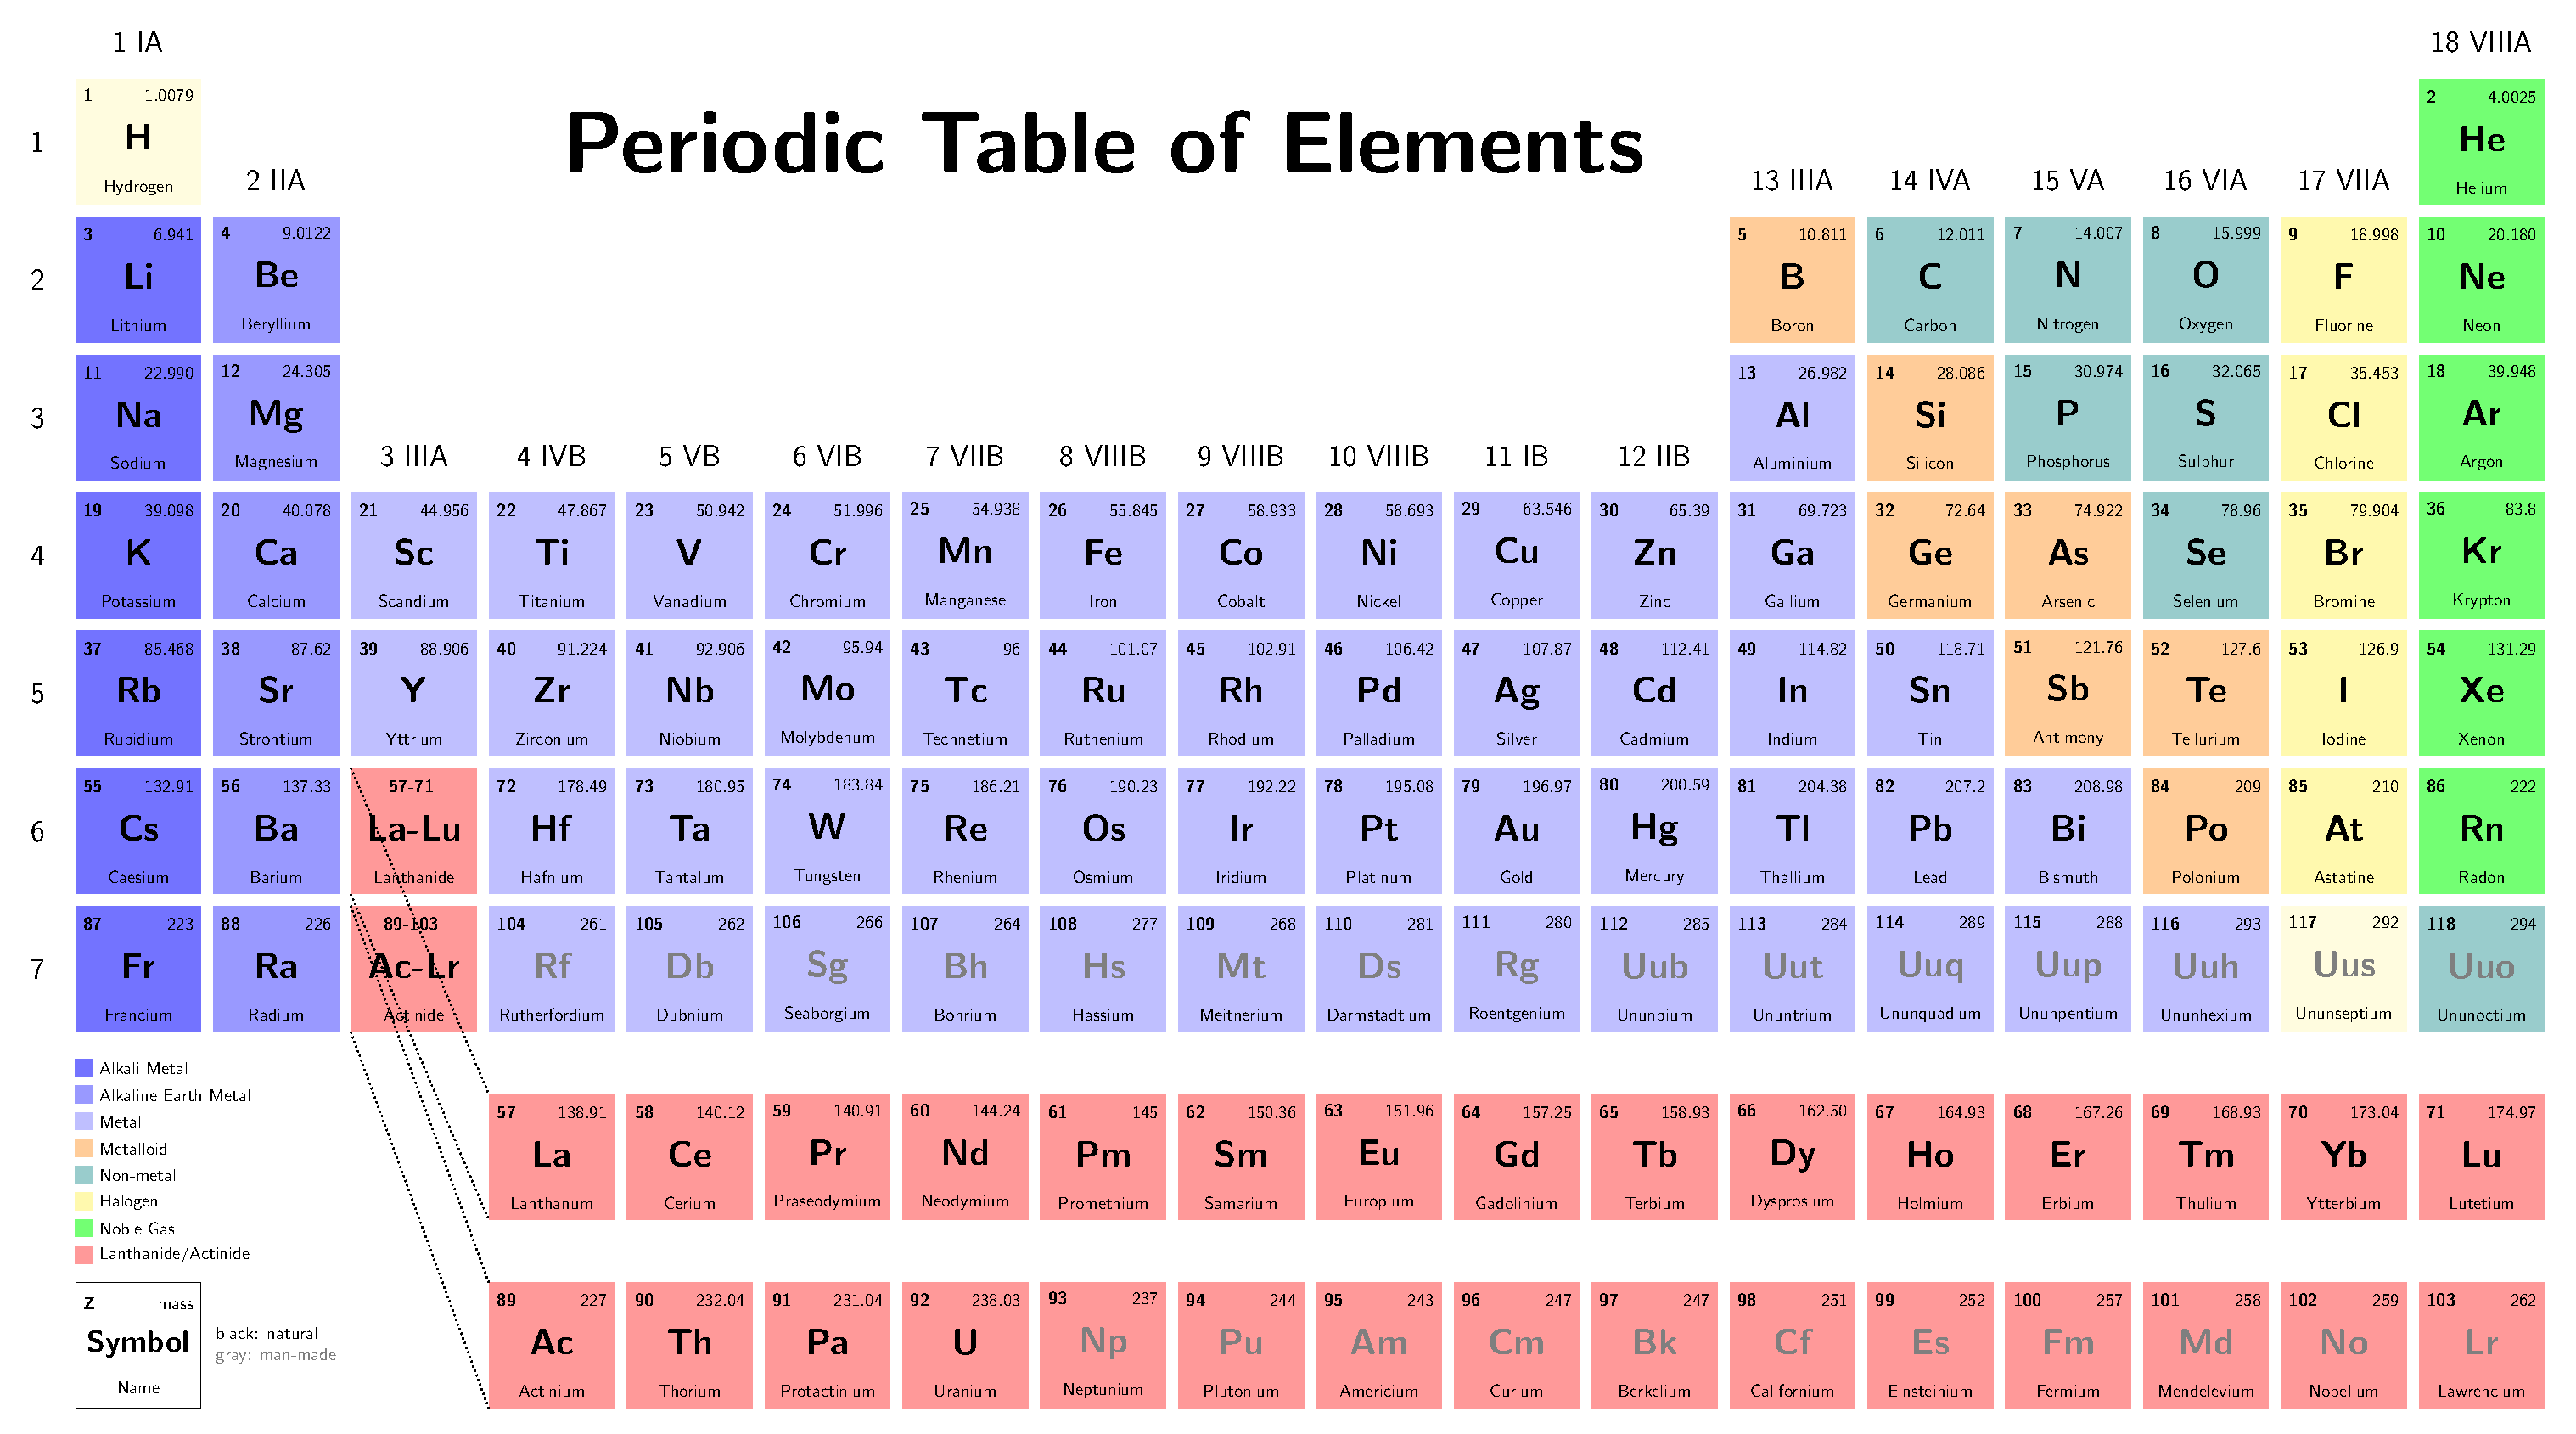
\includepdf[angle=-90]{periodicTable.pdf}
	
\end{document}
